\documentclass{article}

\usepackage{graphicx}

\usepackage[margin=0.1cm]{geometry}

\begin{document}

\begin{figure}
\centering
\includegraphics[width = 0.4\textwidth]{chicr.pdf}
\includegraphics[width = 0.4\textwidth]{chibr.pdf}
\caption{$\chi_{c,b}$ ratios}
\end{figure}

\begin{figure}
\centering
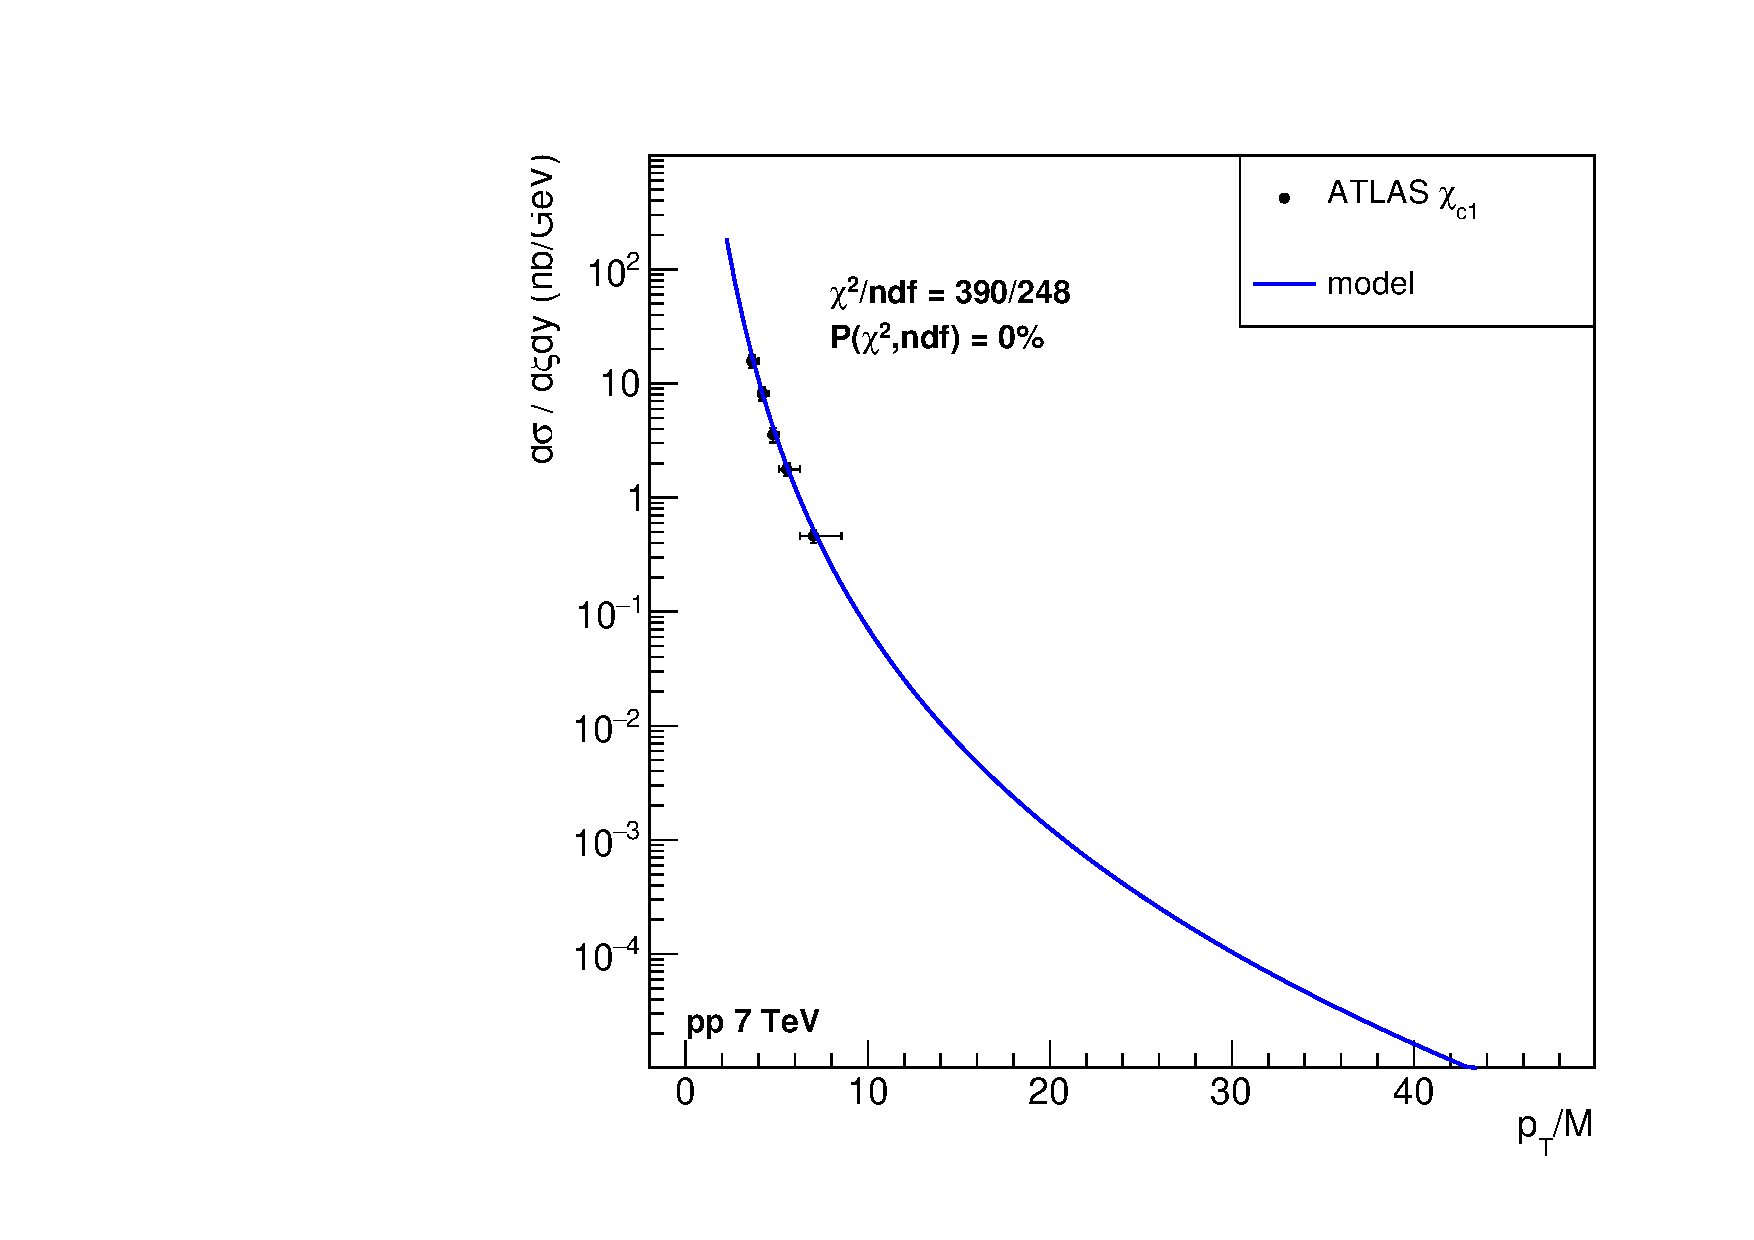
\includegraphics[width = 0.4\textwidth]{chic1_cs.pdf}
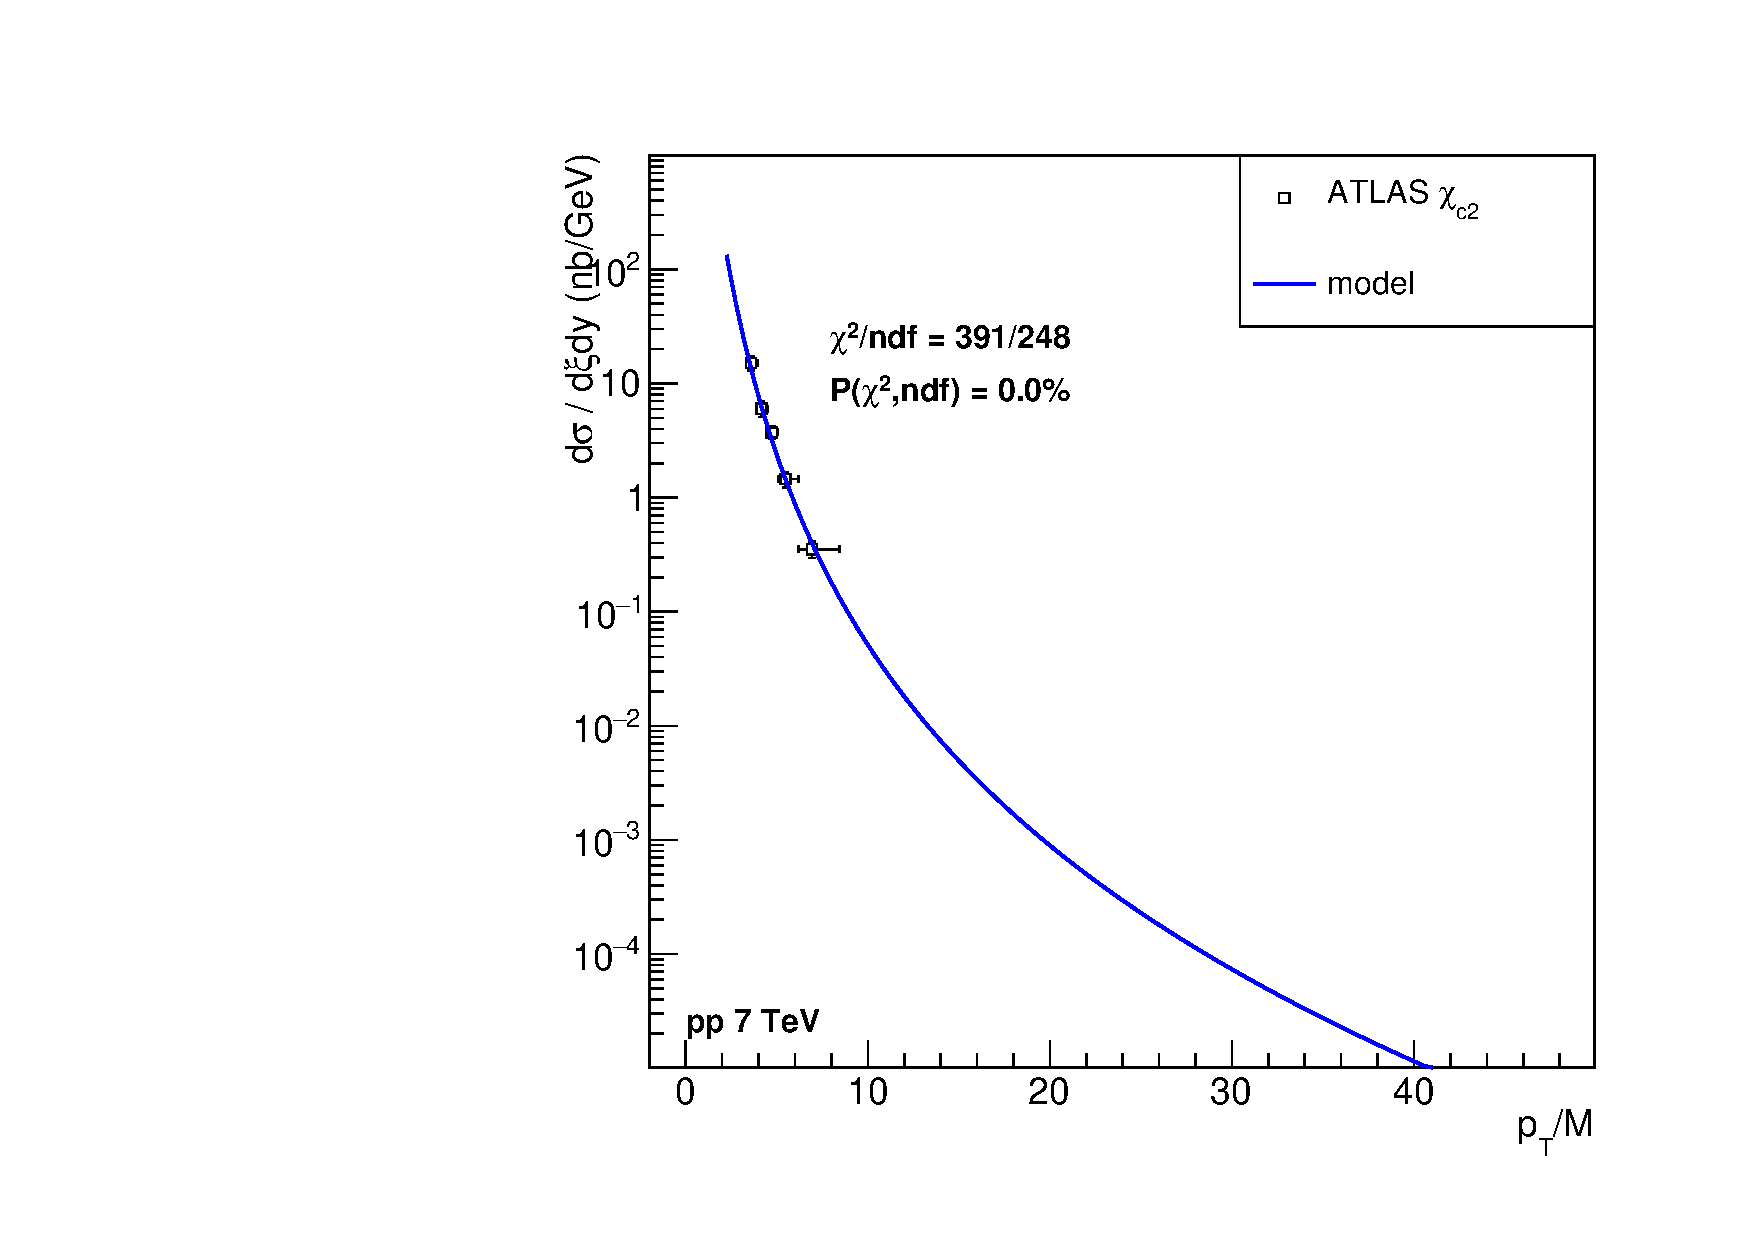
\includegraphics[width = 0.4\textwidth]{chic2_cs.pdf}

\includegraphics[width = 0.4\textwidth]{chic1_cs_pull.pdf}
\includegraphics[width = 0.4\textwidth]{chic2_cs_pull.pdf}
\caption{$\chi_c$ results}
\end{figure}

\clearpage

\begin{figure}
\centering
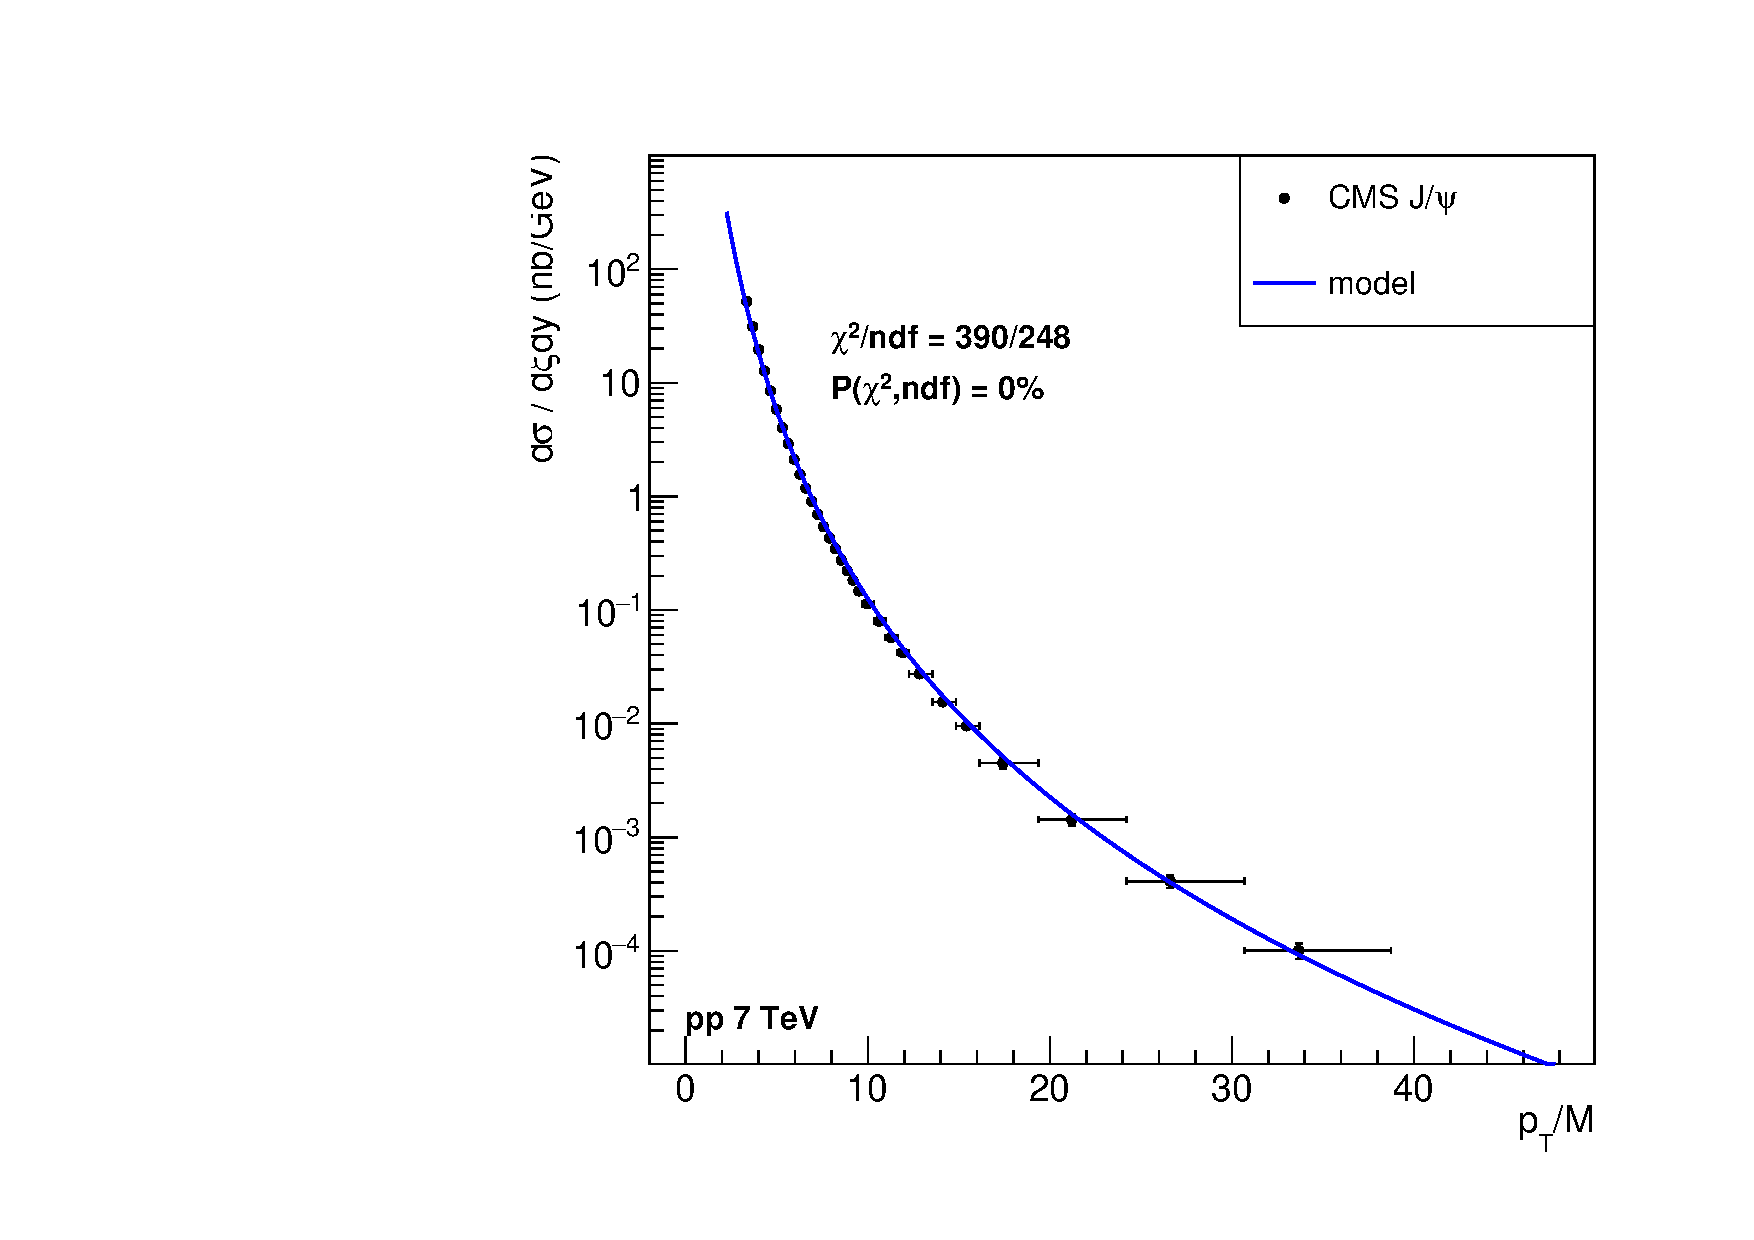
\includegraphics[width = 0.4\textwidth]{jpsi_cs.pdf}
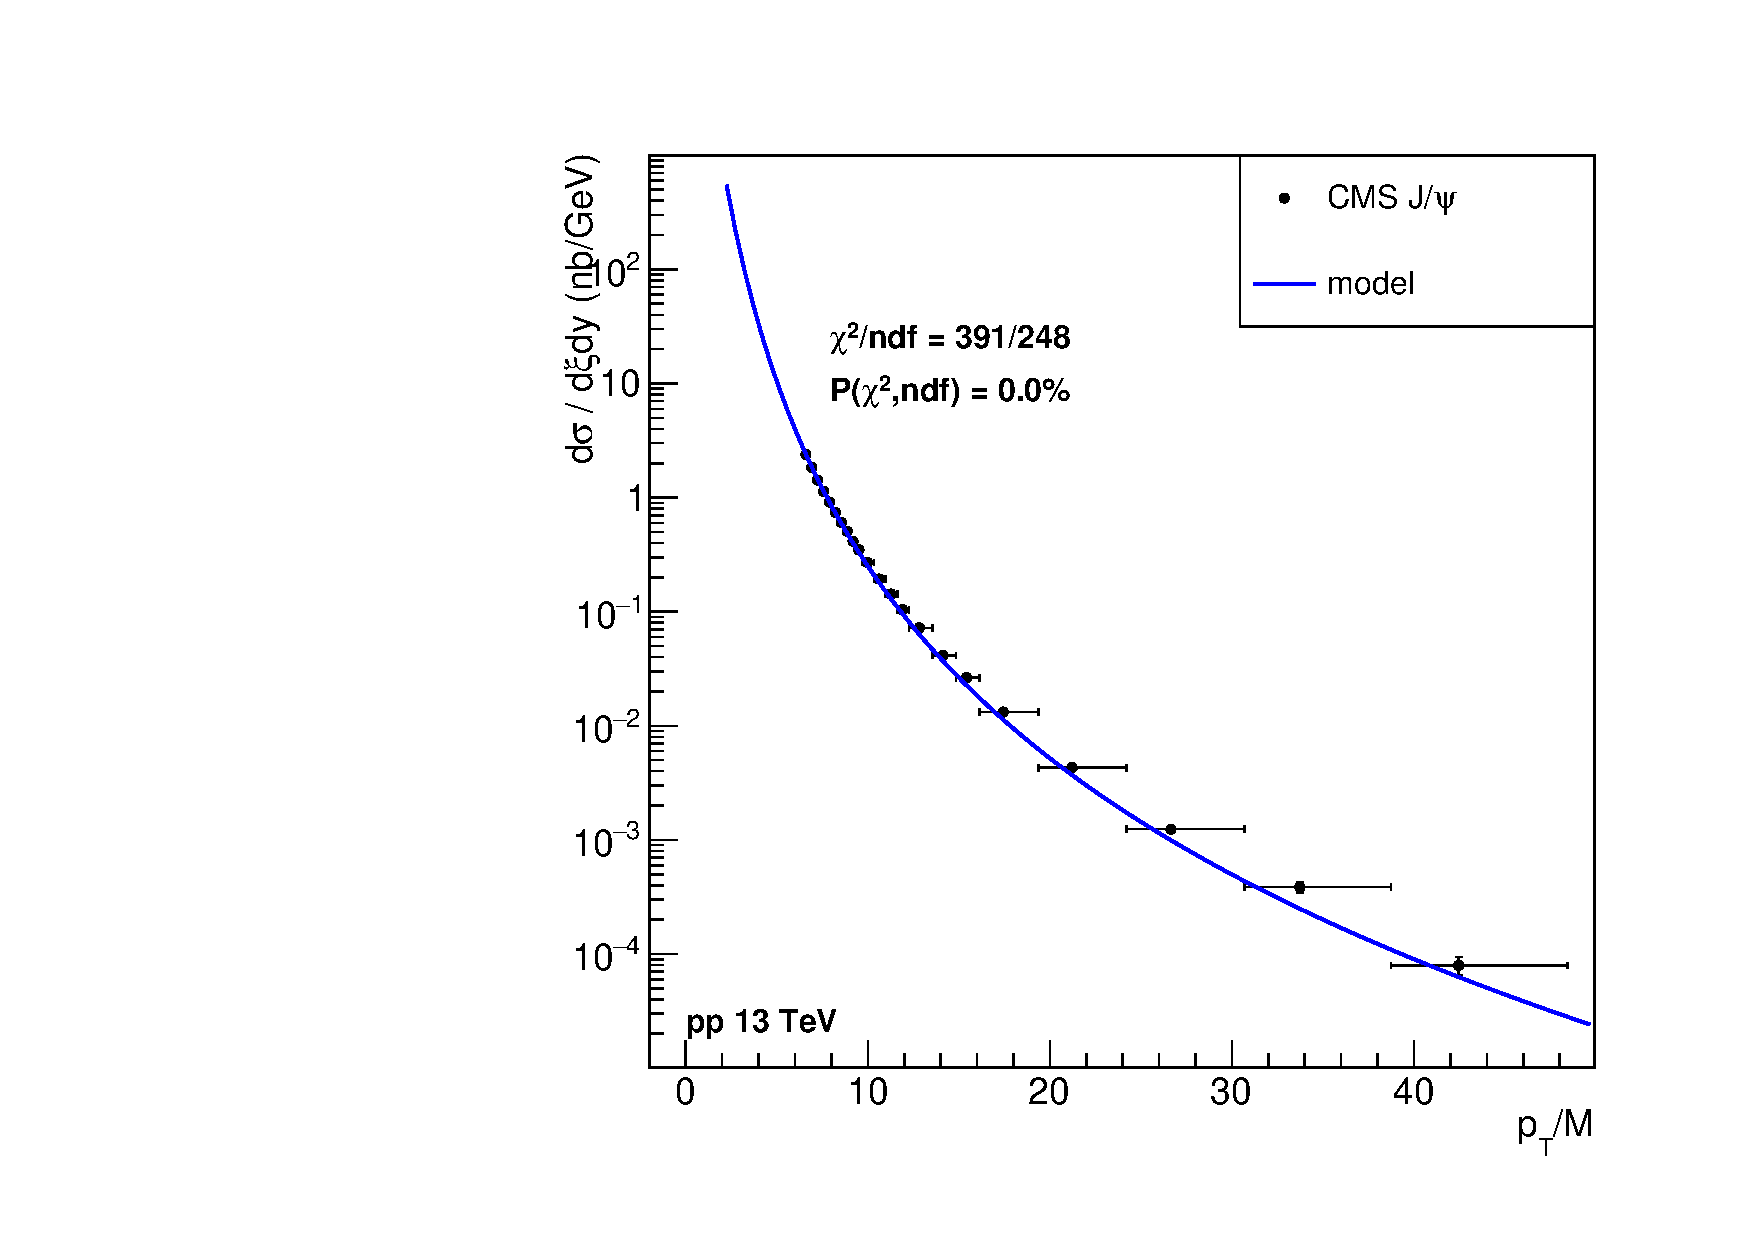
\includegraphics[width = 0.4\textwidth]{jpsi_13_cs.pdf}

\includegraphics[width = 0.4\textwidth]{jpsi_cs_pull.pdf}
\includegraphics[width = 0.4\textwidth]{jpsi_13_cs_pull.pdf}
\caption{J/$\psi$ results}
\end{figure}

\clearpage

\begin{figure}
\centering
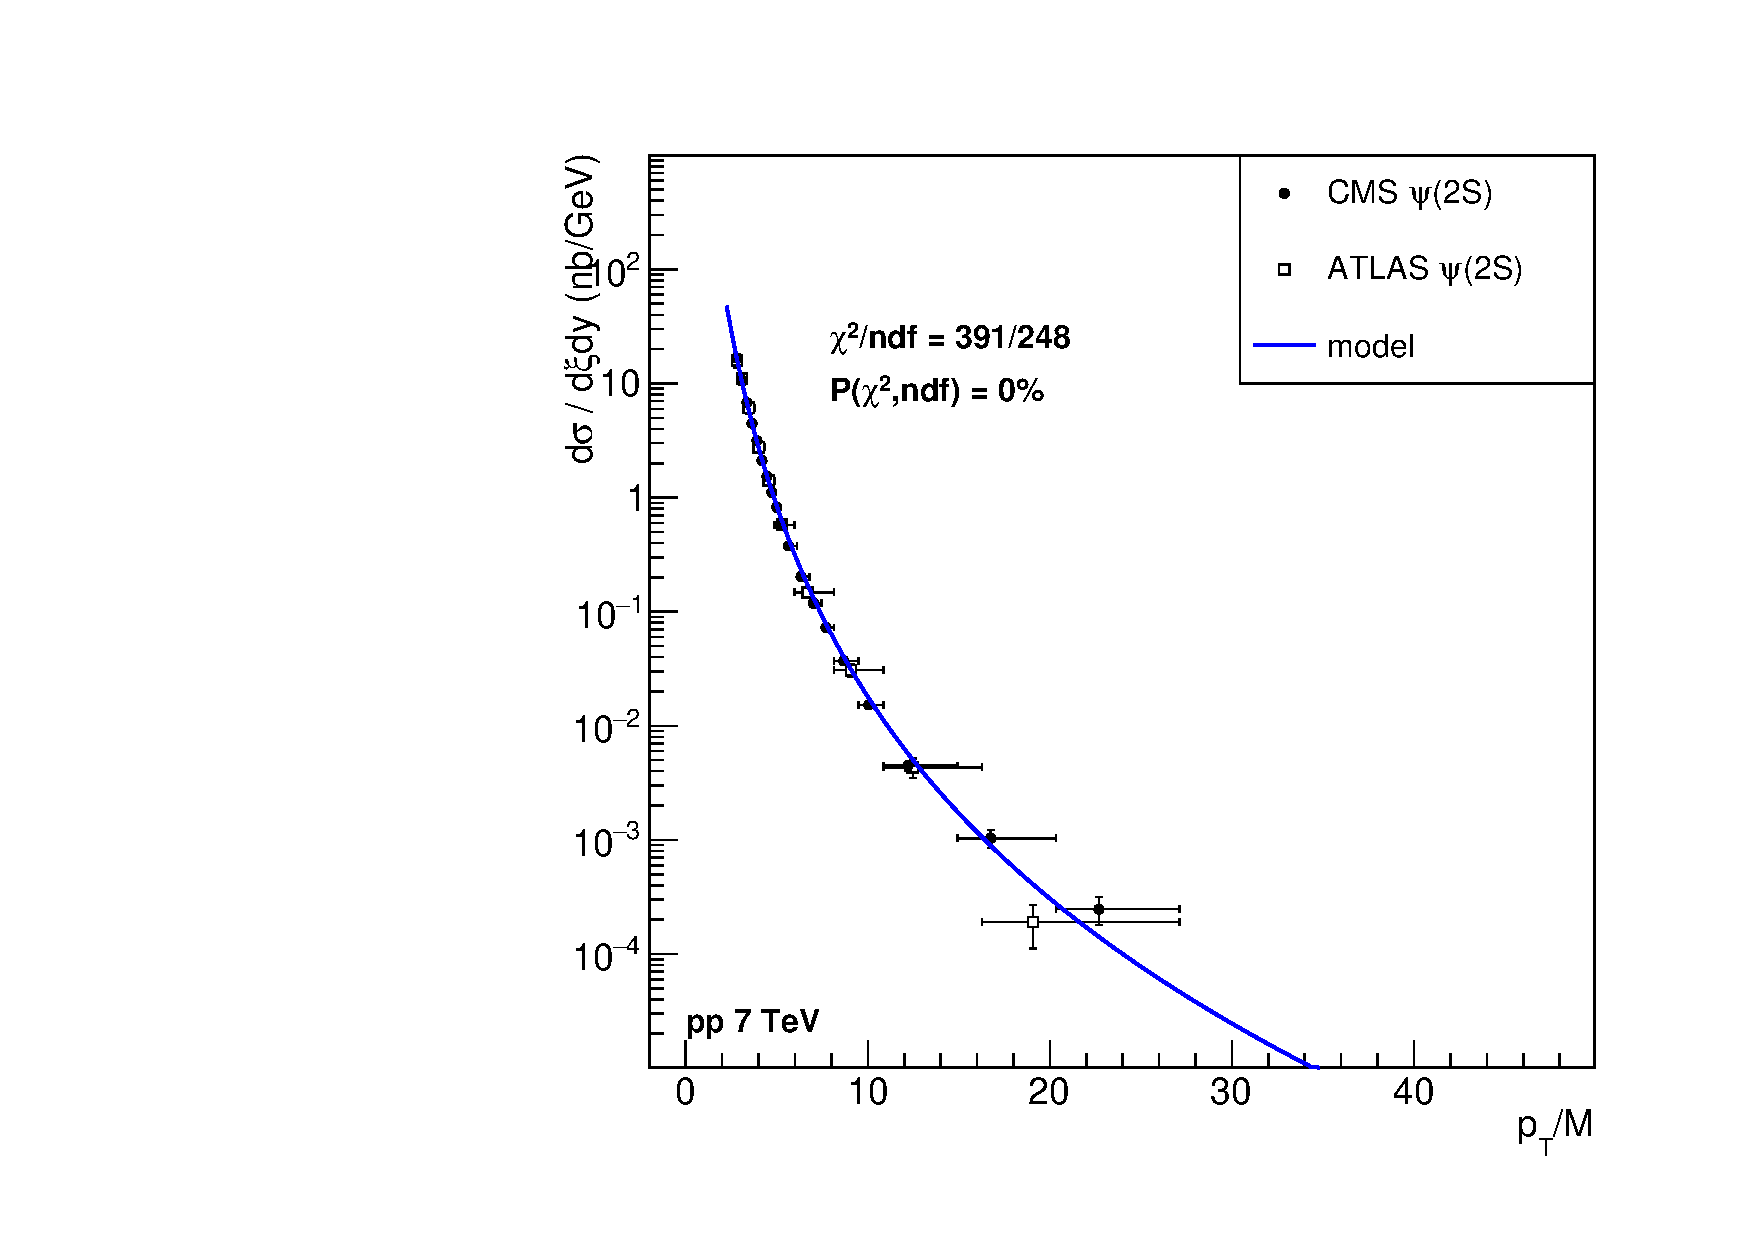
\includegraphics[width = 0.4\textwidth]{psiprime_cs.pdf}
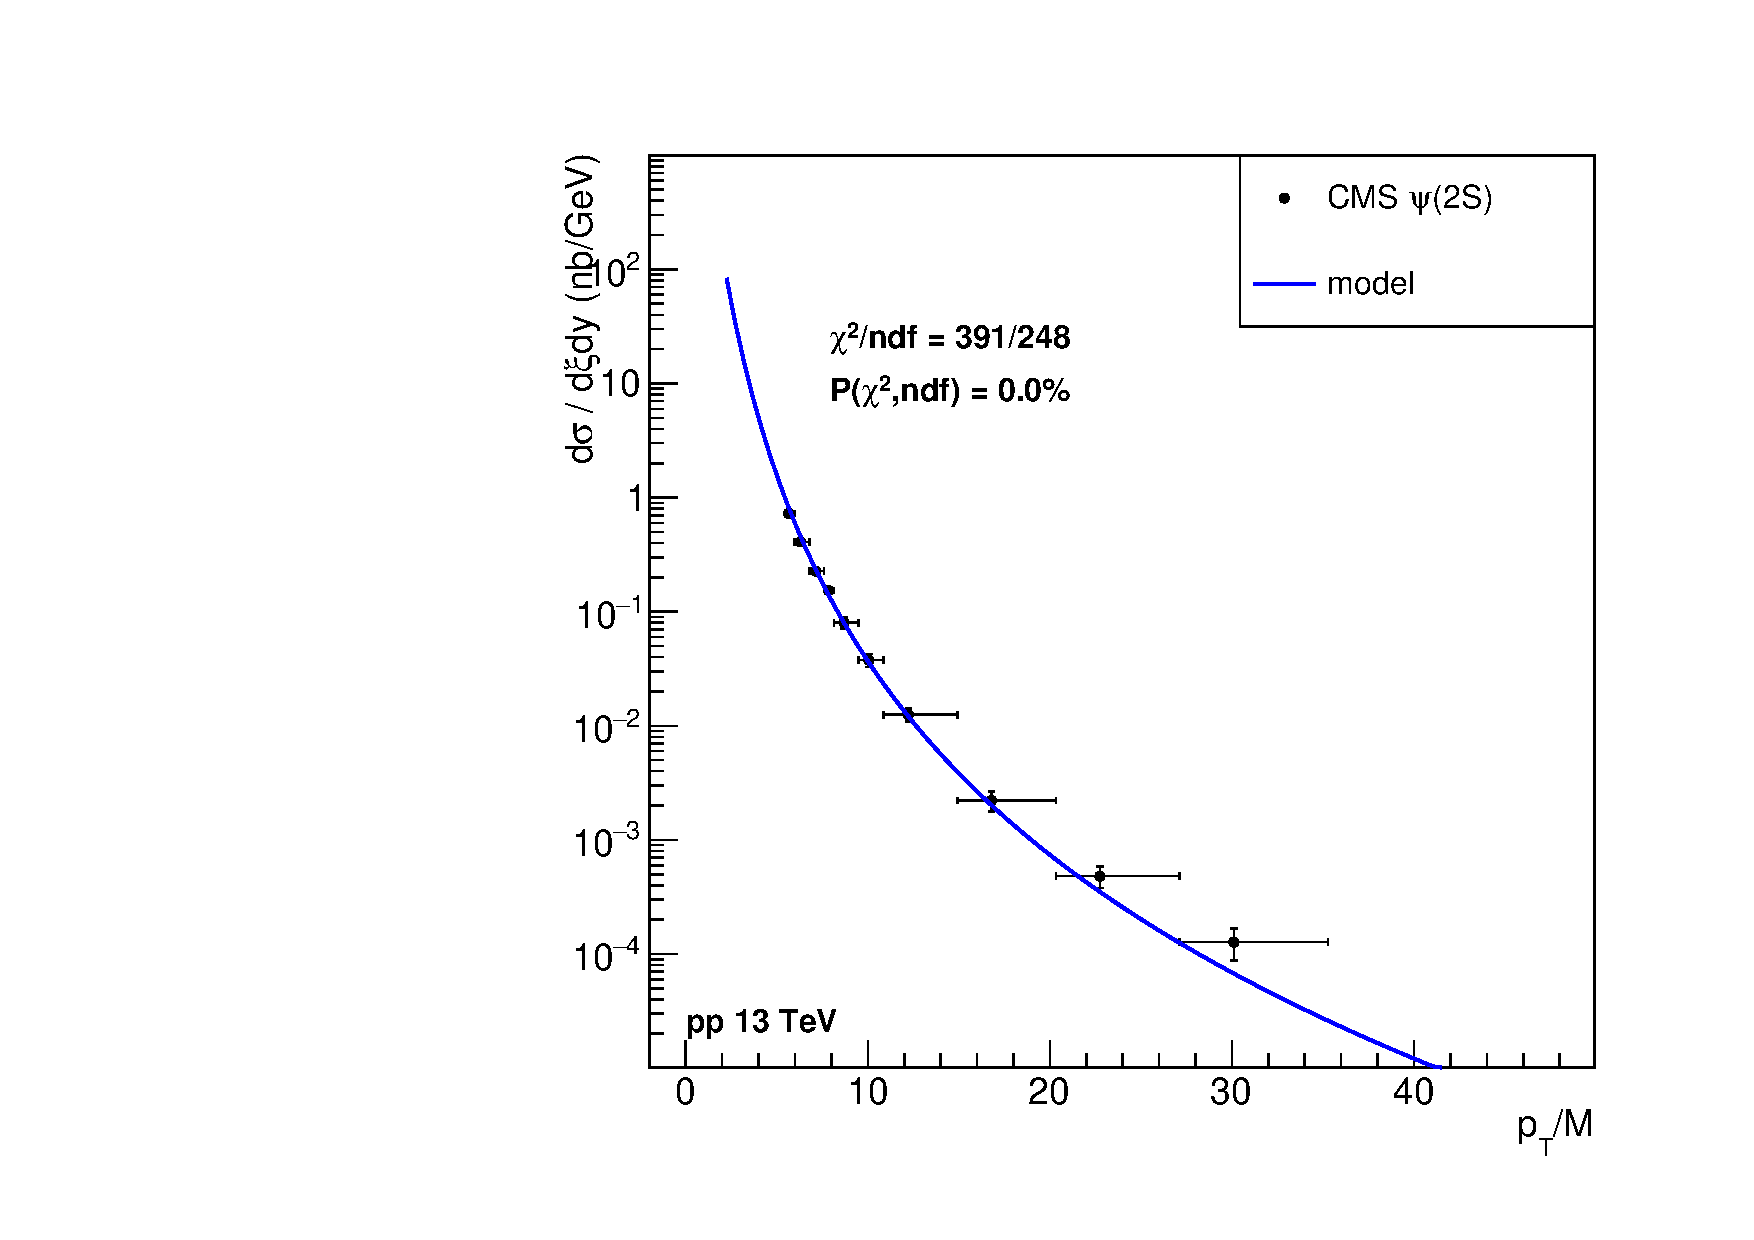
\includegraphics[width = 0.4\textwidth]{psiprime_13_cs.pdf}

\includegraphics[width = 0.4\textwidth]{psiprime_cs_pull.pdf}
\includegraphics[width = 0.4\textwidth]{psiprime_13_cs_pull.pdf}
\caption{$\psi(2S)$ results}
\end{figure}

\clearpage

\begin{figure}
\centering
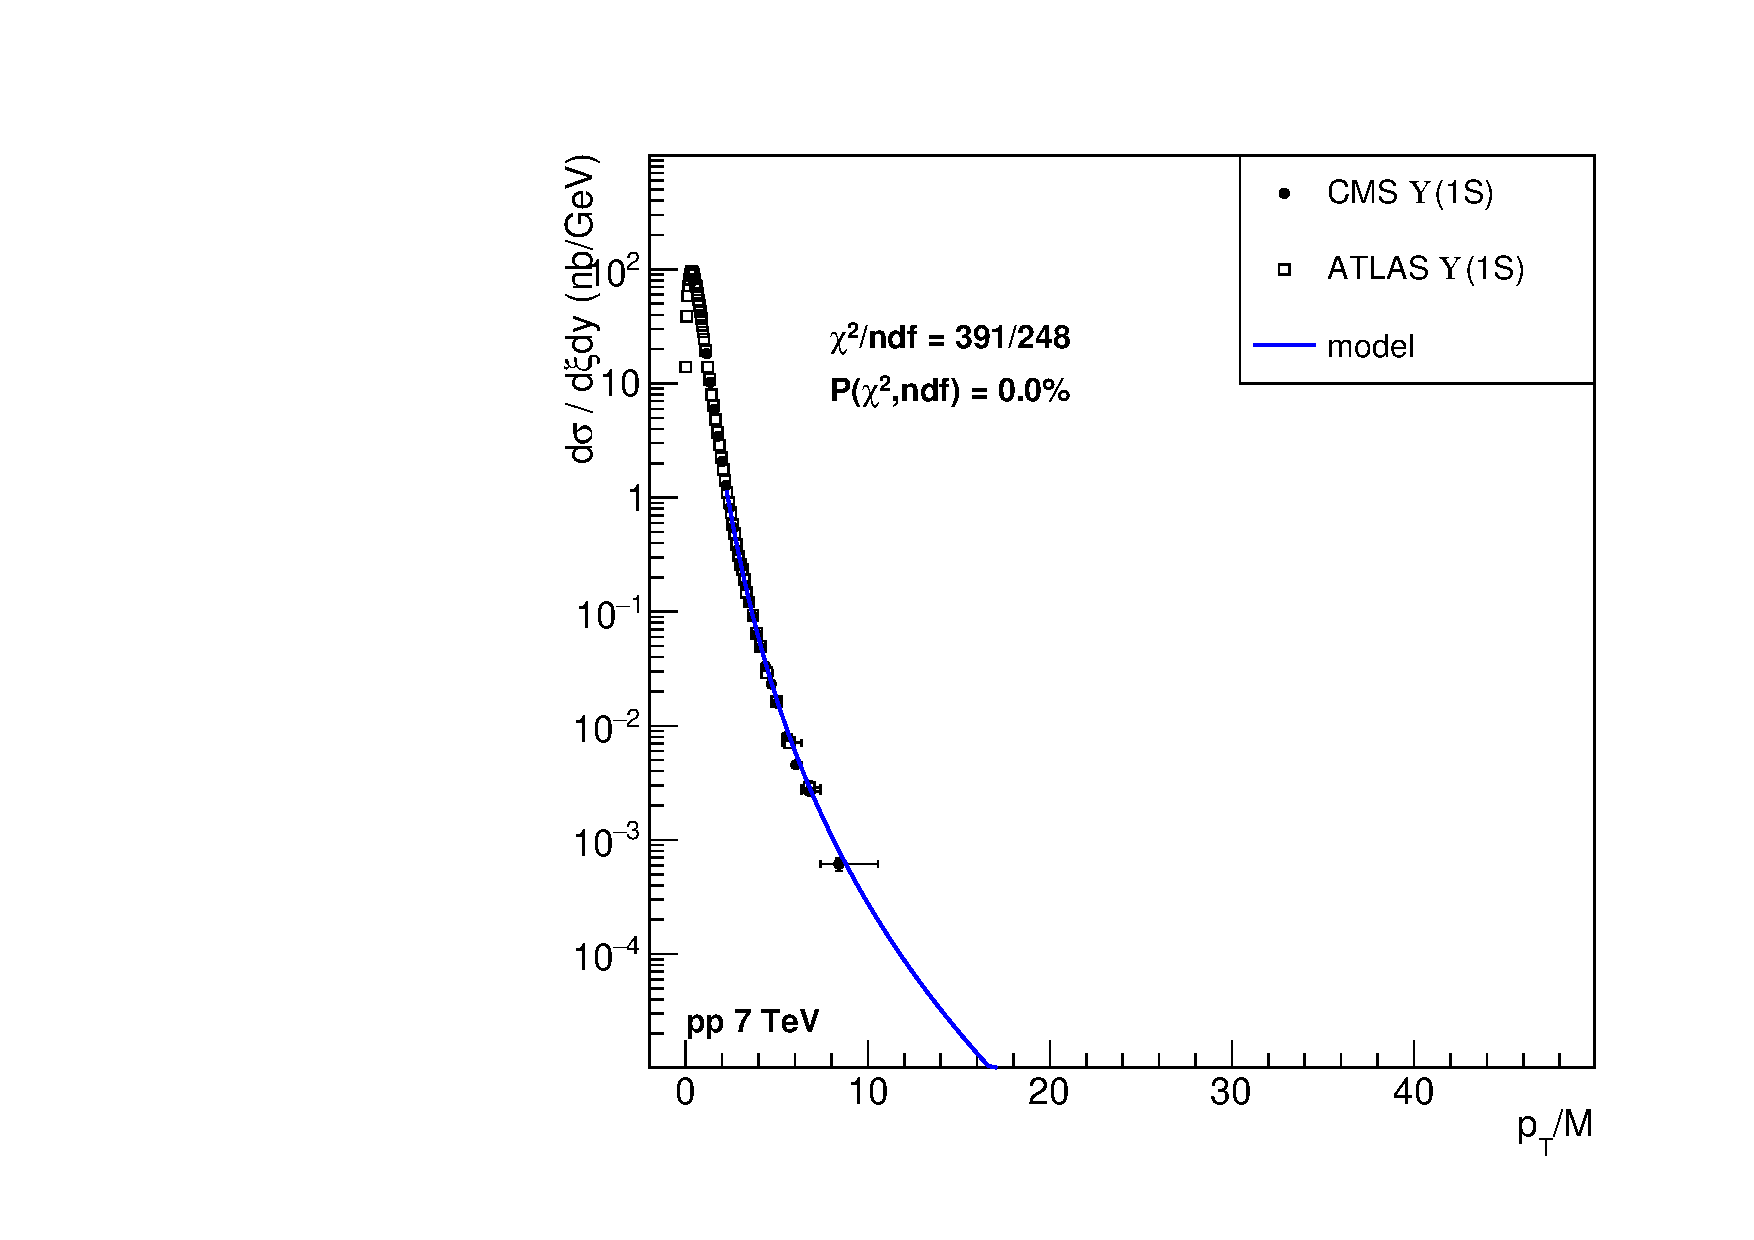
\includegraphics[width = 0.4\textwidth]{ups1S_cs.pdf}
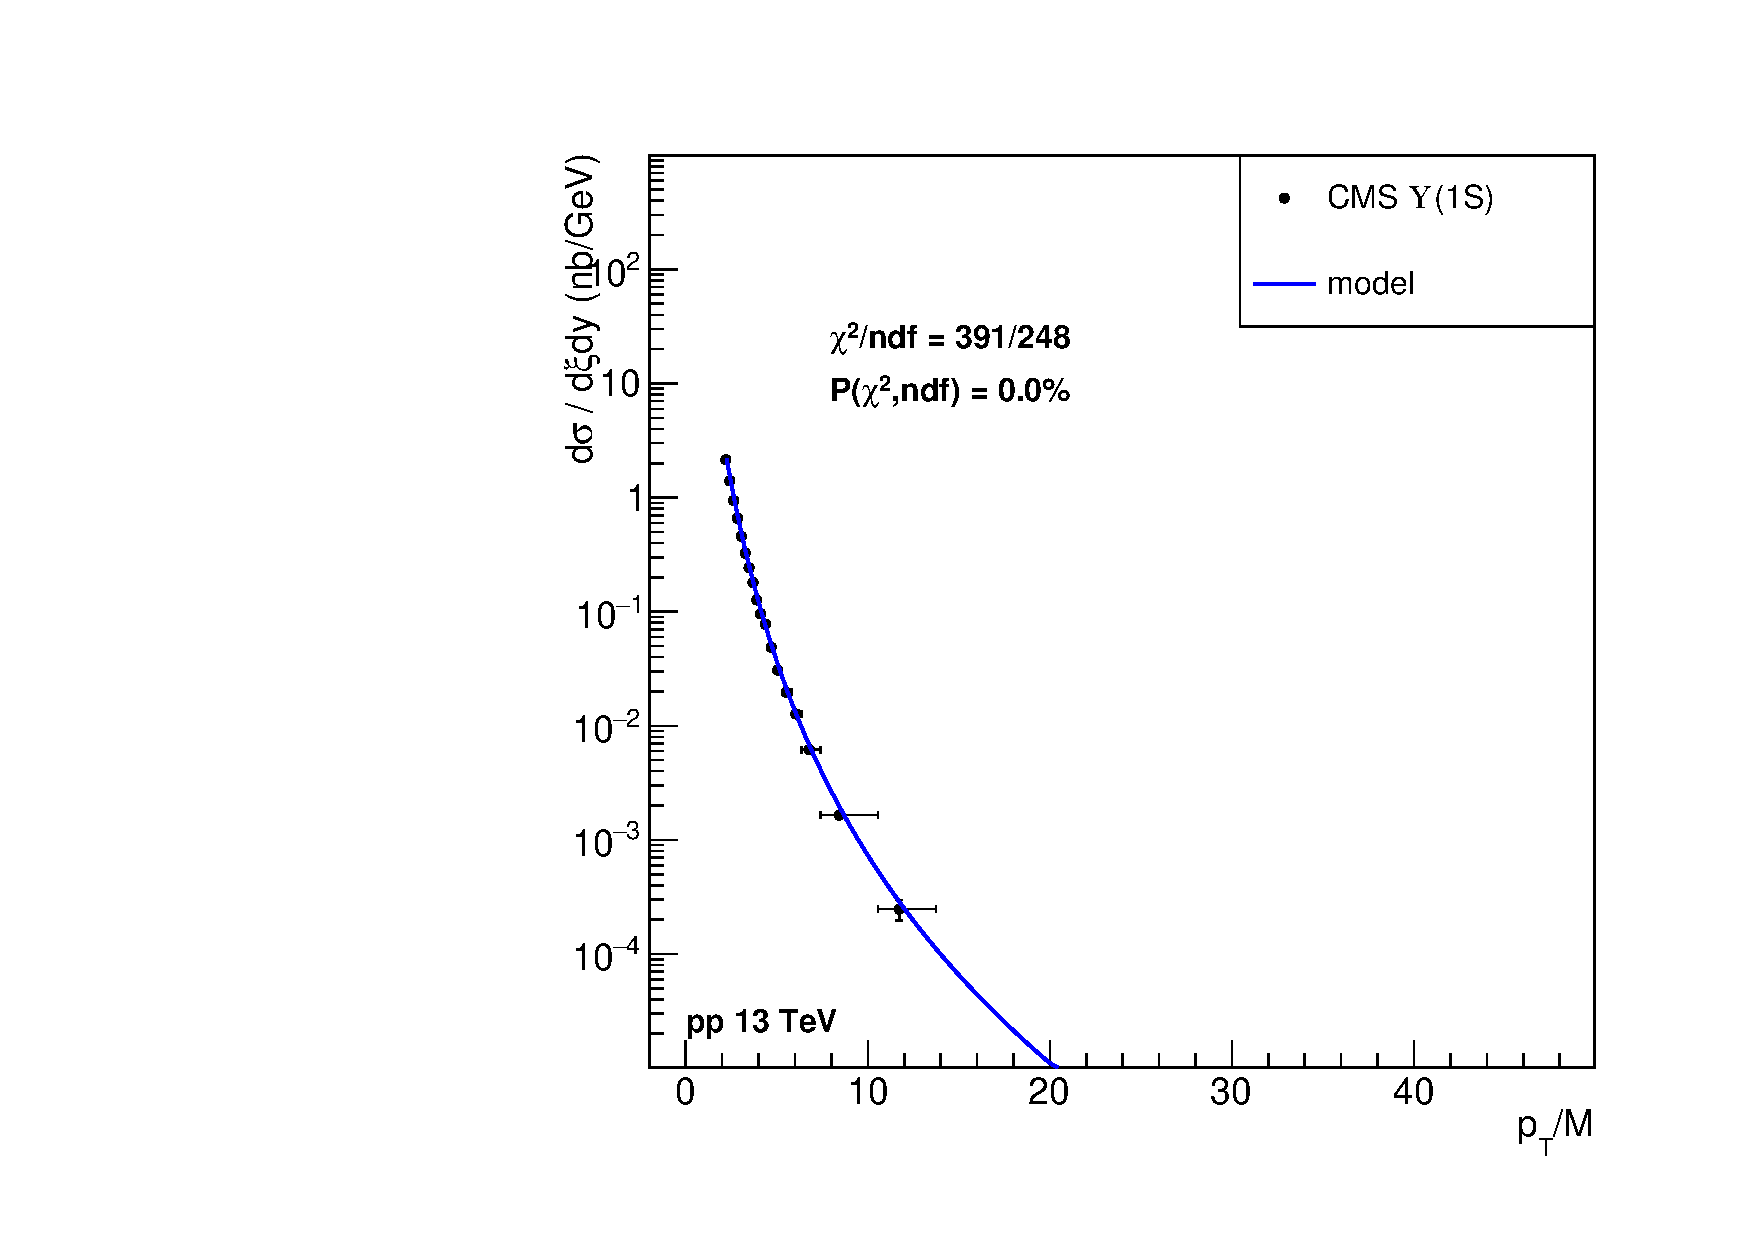
\includegraphics[width = 0.4\textwidth]{ups1S_13_cs.pdf}

\includegraphics[width = 0.4\textwidth]{ups1S_cs_pull.pdf}
\includegraphics[width = 0.4\textwidth]{ups1S_13_cs_pull.pdf}
\caption{$\Upsilon(1S)$ results}
\end{figure}

\clearpage

\begin{figure}
\centering
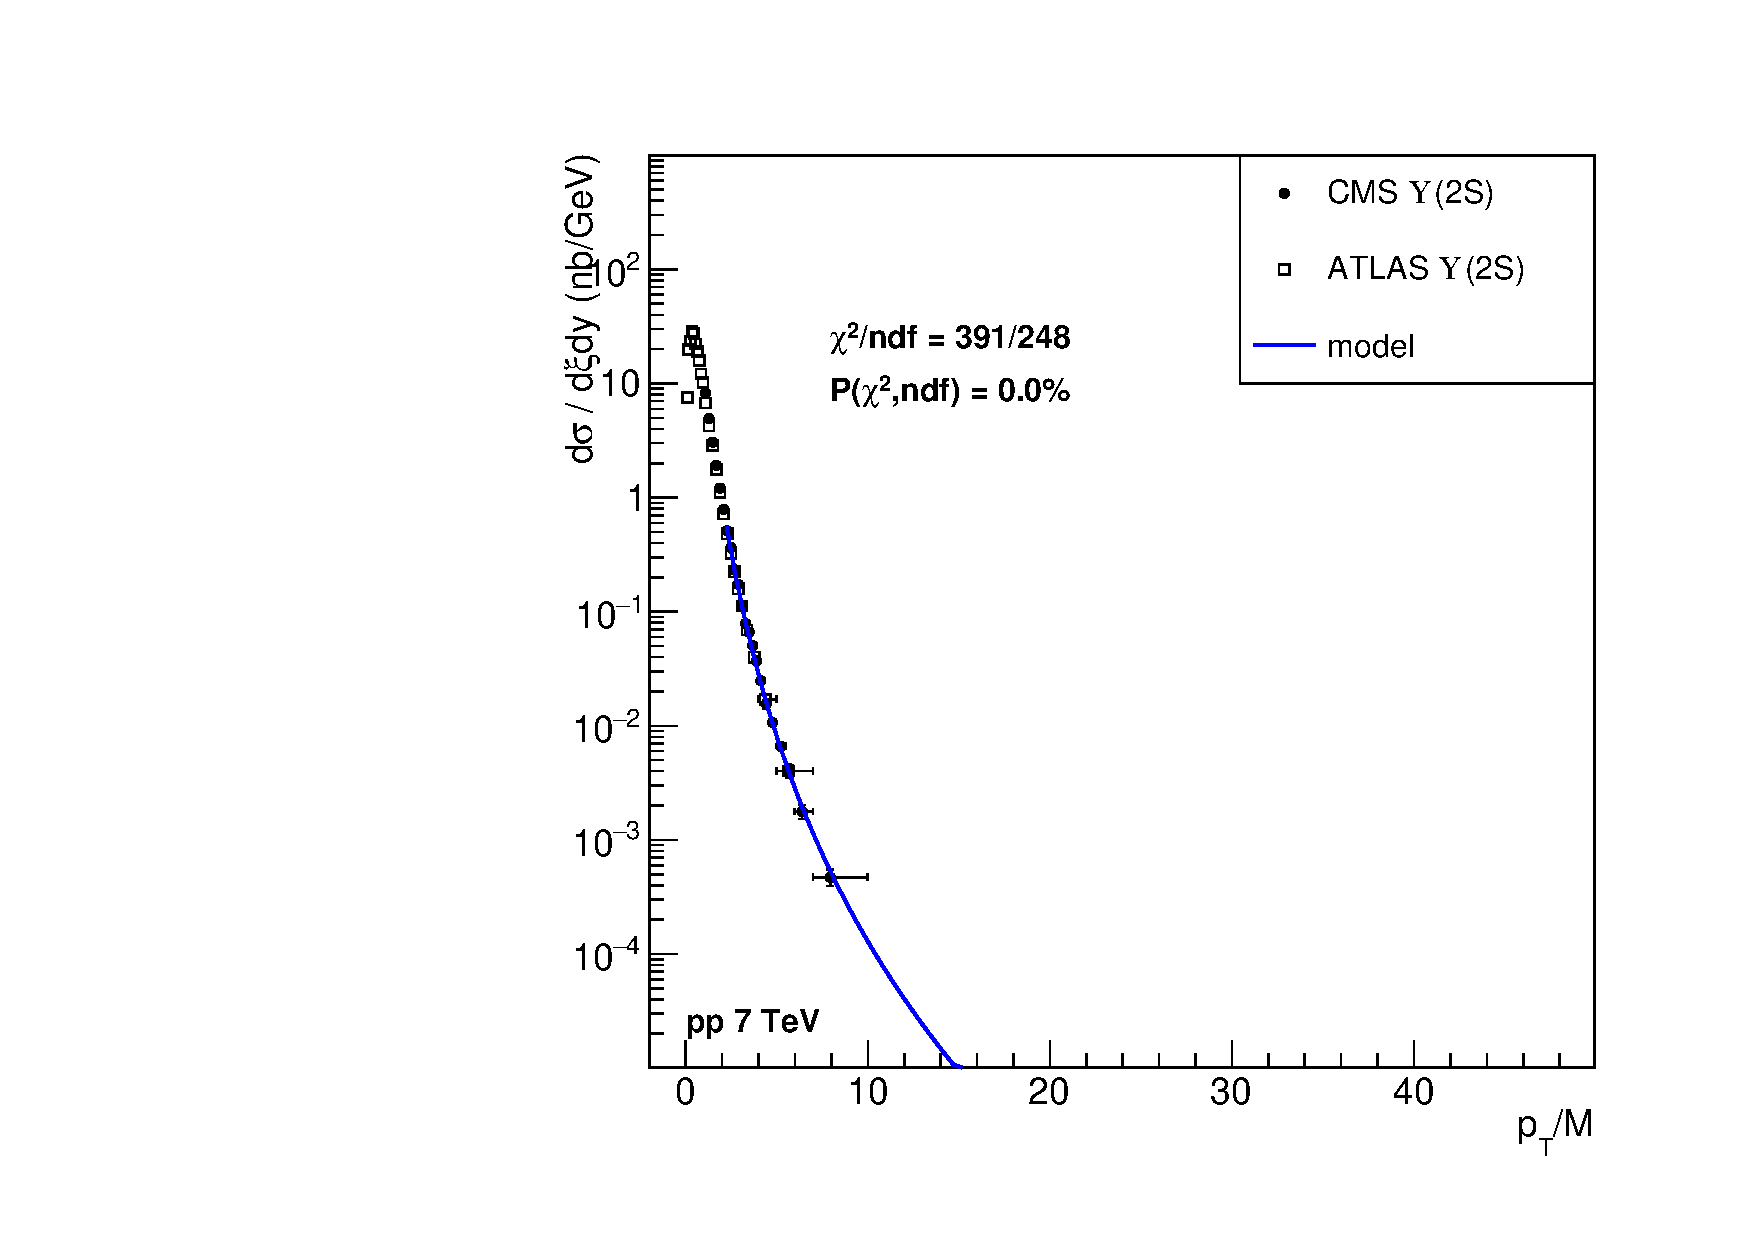
\includegraphics[width = 0.4\textwidth]{ups2S_cs.pdf}
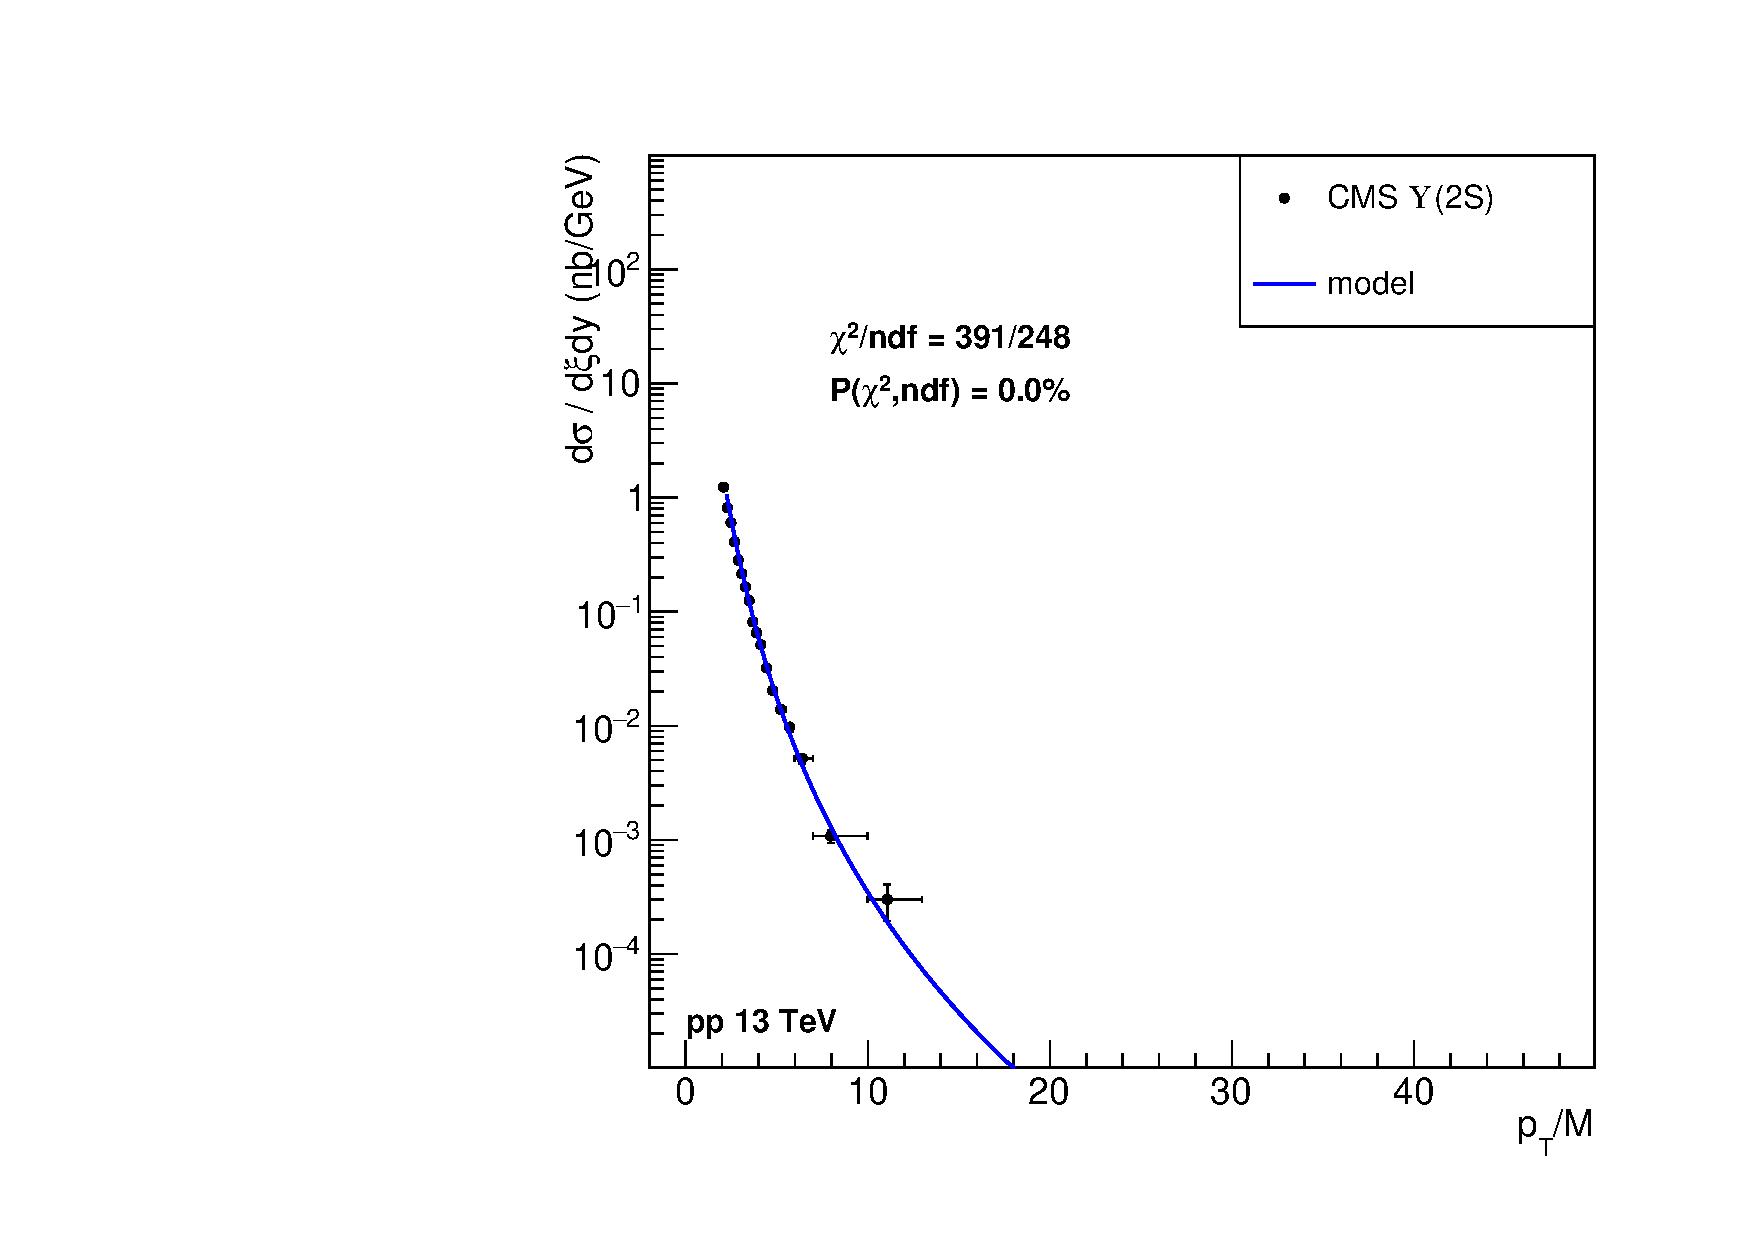
\includegraphics[width = 0.4\textwidth]{ups2S_13_cs.pdf}

\includegraphics[width = 0.4\textwidth]{ups2S_cs_pull.pdf}
\includegraphics[width = 0.4\textwidth]{ups2S_13_cs_pull.pdf}
\caption{$\Upsilon(2S)$ results}
\end{figure}

\clearpage

\begin{figure}
\centering
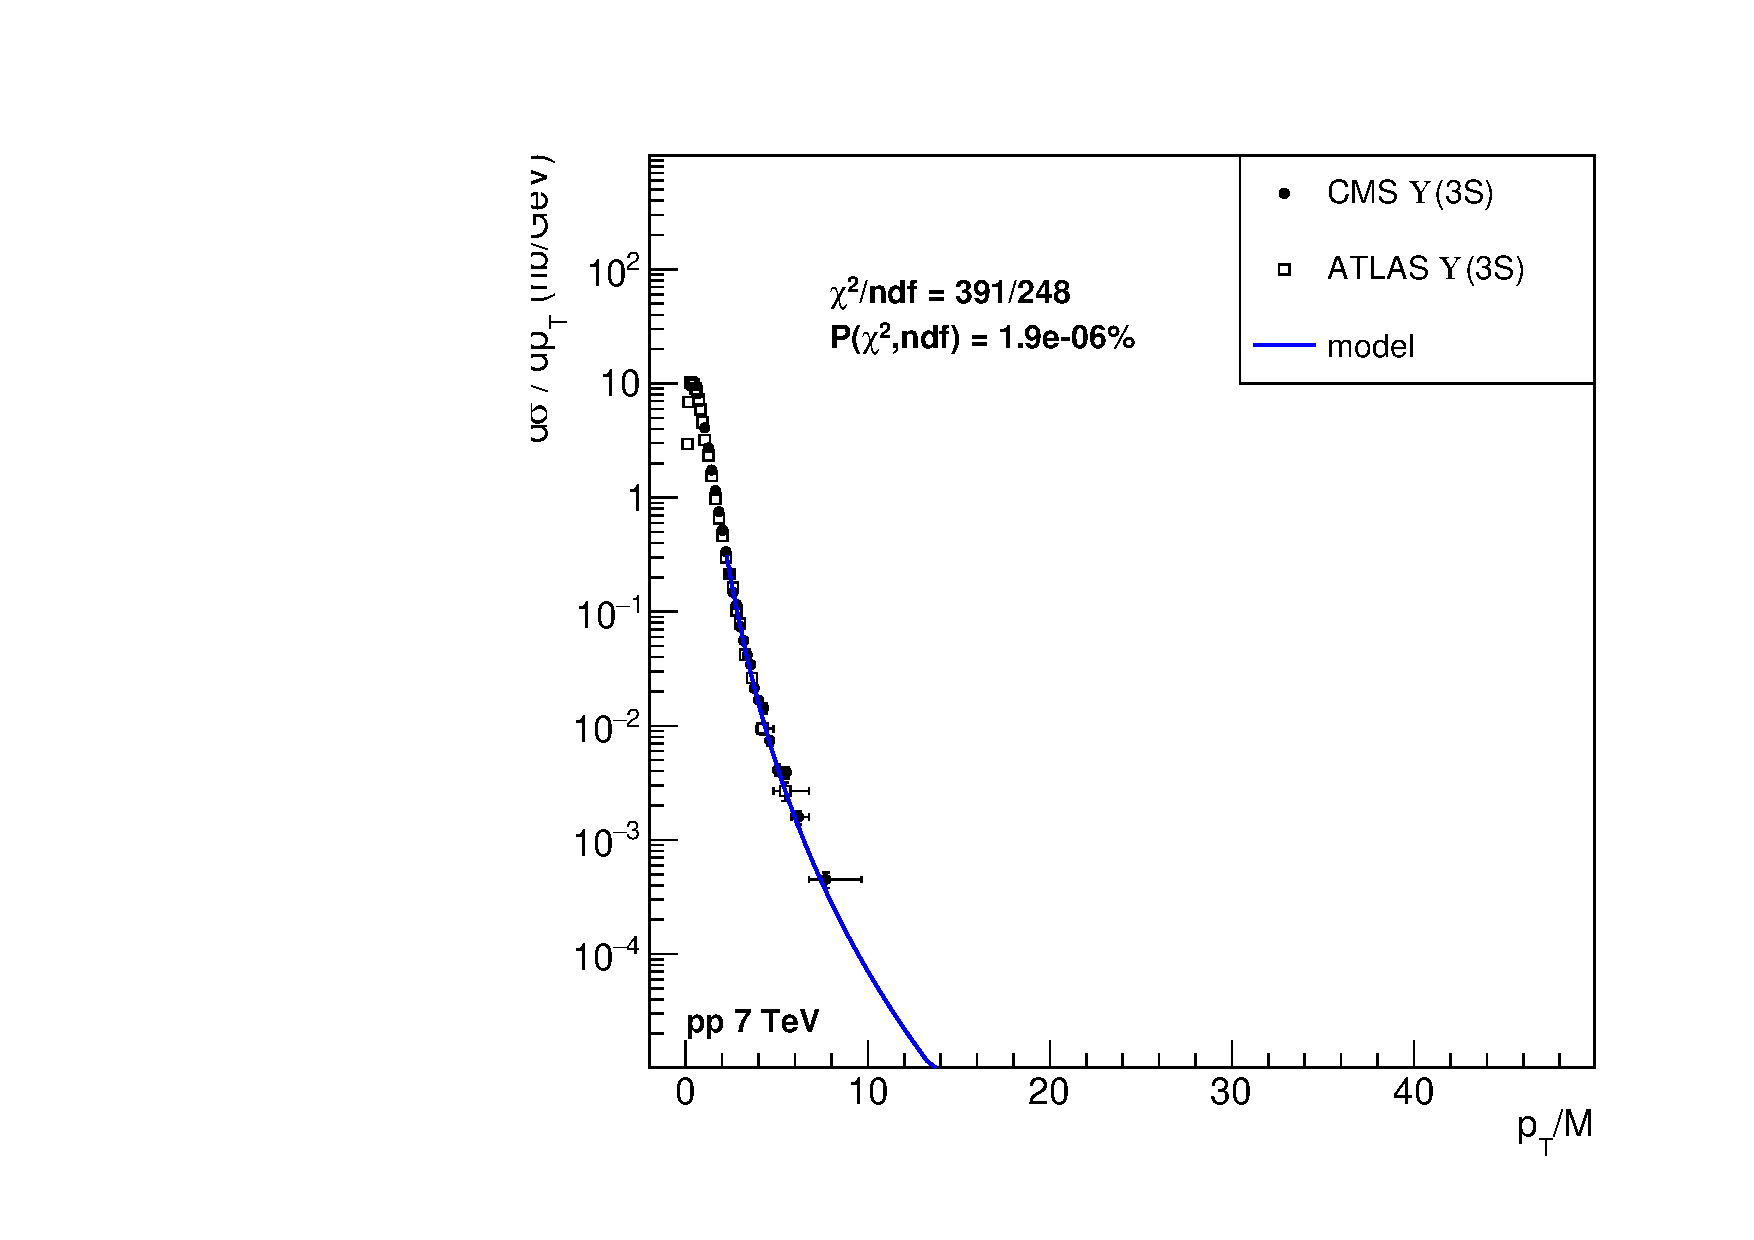
\includegraphics[width = 0.4\textwidth]{ups3S_cs.pdf}
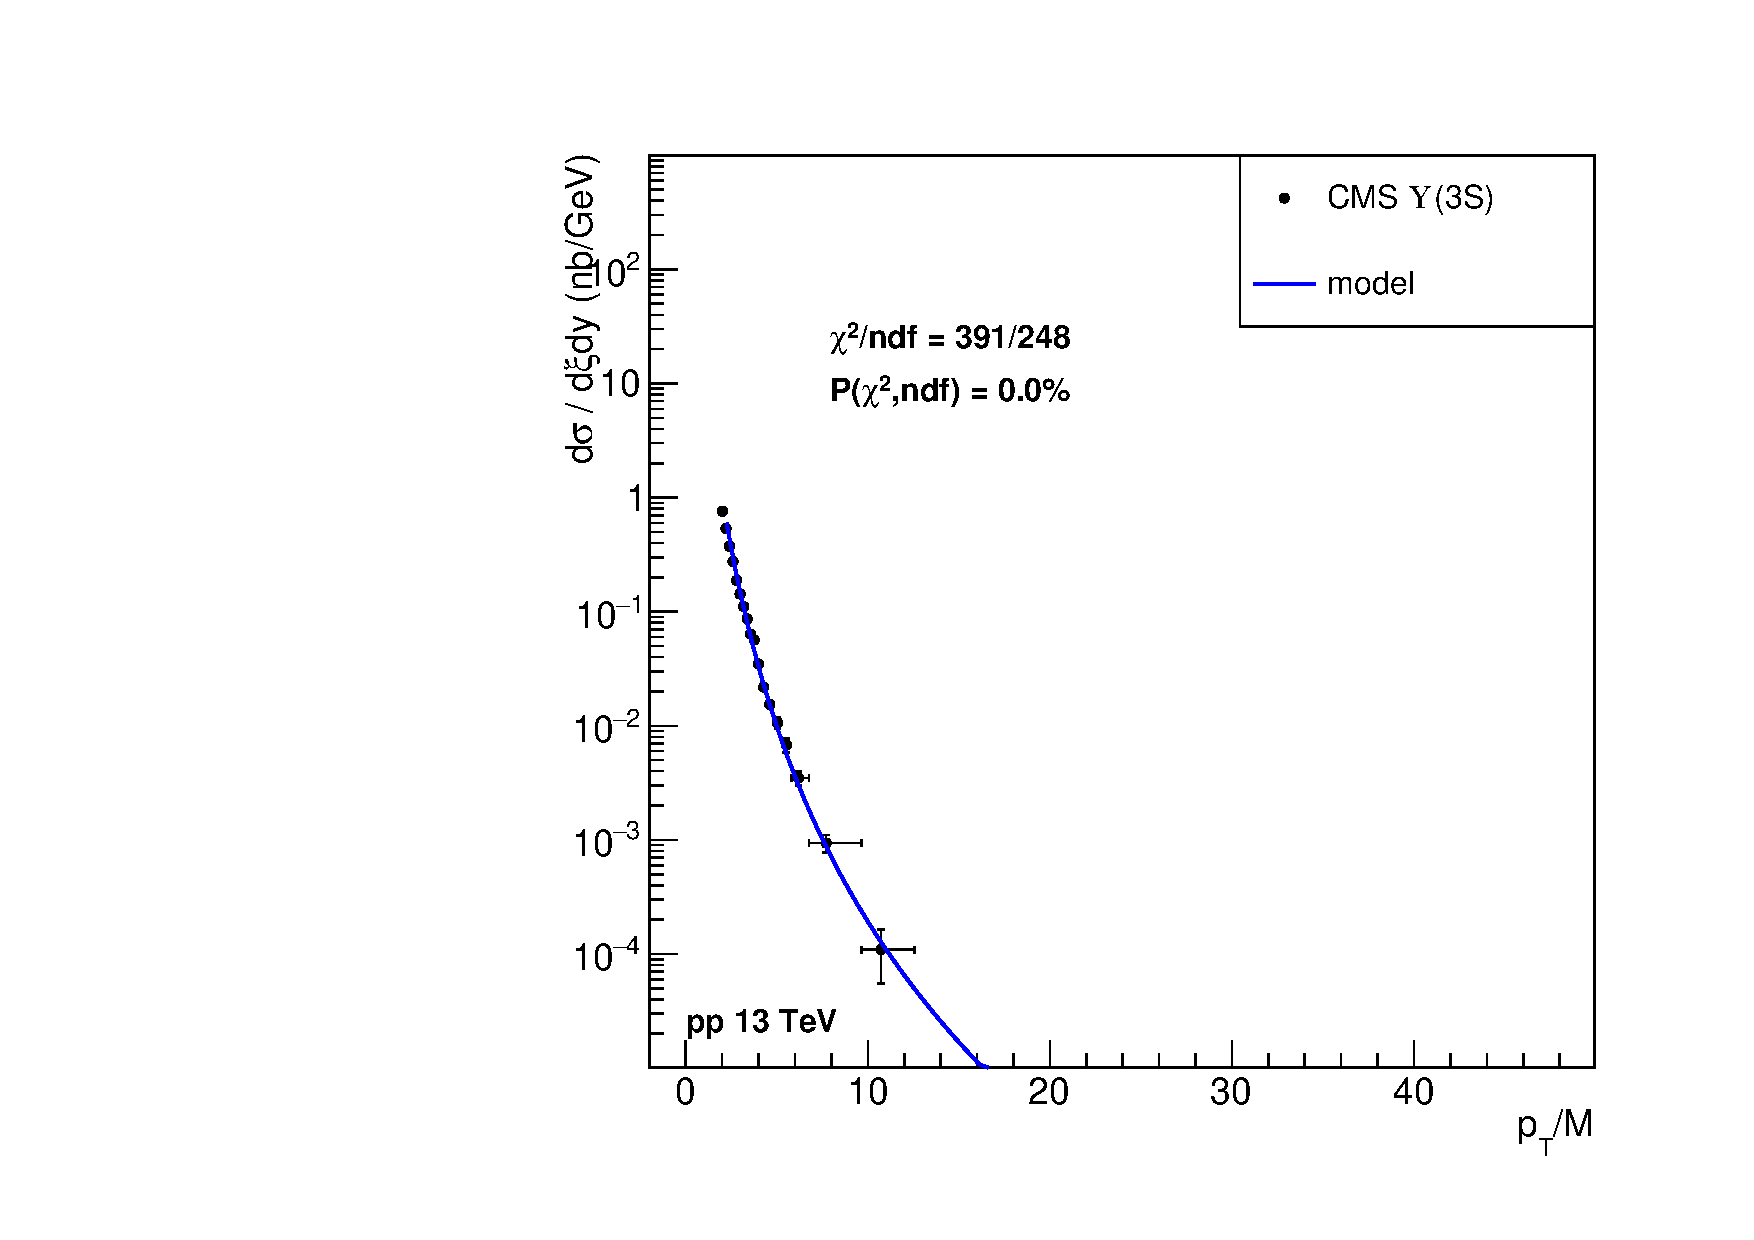
\includegraphics[width = 0.4\textwidth]{ups3S_13_cs.pdf}

\includegraphics[width = 0.4\textwidth]{ups3S_cs_pull.pdf}
\includegraphics[width = 0.4\textwidth]{ups3S_13_cs_pull.pdf}
\caption{$\Upsilon(3S)$ results}
\end{figure}

\clearpage

\begin{table}[h!]
\centering
\begin{tabular}{c|c|c}
Parameter & Value & Uncertainty \\
\hline
$L_{J/\psi}$ & 0.6580 & 0.0084 \\
$L_{\chi_{c1}}$ & 0.671 & 0.071 \\
$L_{\chi_{c2}}$ & 0.640 & 0.033 \\
$L_{\psi(2S)}$ & 0.2545 & 0.0077 \\
$L_{\Upsilon(1S)}$ & 1.710 & 0.021 \\
$L_{\Upsilon(2S)}$ & 1.203 & 0.018 \\
$L_{\Upsilon(3S)}$ & 0.855 & 0.014 \\
$\rho$ & 2.0 & fixed \\
$\delta$ & 0.0 & fixed \\
$\beta_{J/\psi}$ & 2.8060 & 0.0046 \\
$\beta_{\chi_{c1}}$ & 2.79 & 0.14 \\
$\beta_{\chi_{c2}}$ & 2.931 & 0.053 \\
$\beta_{\psi(2S)}$ & 2.8258 & 0.0093 \\
$\beta_{\Upsilon(1S)}$ & 2.768 & 0.015 \\
$\beta_{\Upsilon(2S)}$ & 2.713 & 0.025 \\
$\beta_{\Upsilon(3S)}$ & 2.636 & 0.030 \\
$BR(J/\psi\rightarrow\mu^+\mu^-)$ & 1.0005 & 0.0055 (0.0841 $\sigma$) \\
$BR(\chi_{c1}\rightarrow J/\psi\gamma)$ & 1.0 & fixed \\
$BR(\chi_{c2}\rightarrow J/\psi\gamma)$ & 1.0 & fixed \\
$BR(\psi(2S)\rightarrow\mu^+\mu^-)$ & 0.906 & 0.029 (-1.259 $\sigma$) \\
$BR(\psi(2S)\rightarrow J/\psi\pi^+\pi^-)$ & 1.0011 & 0.0081 (0.1311 $\sigma$) \\
$\mathcal L_{ATLAS,5.02}$ & 0.997 & 0.018 (-0.062 $\sigma$) \\
$\mathcal L_{ATLAS,7}(c\overline c)$ & 1.005 & 0.016 (0.272 $\sigma$) \\
$\mathcal L_{ATLAS,7}(b\overline b)$ & 1.013 & 0.014 (0.321 $\sigma$) \\
$\mathcal L_{CDF,1.96}(J/\psi)$ & 0.789 & 0.019 (-3.063 $\sigma$) \\
$\mathcal L_{CDF,1.96}(\psi(2S))$ & 0.989 & 0.034 (-0.185 $\sigma$) \\
$\mathcal L_{CMS,5.02}$ & 1.009 & 0.014 (0.407 $\sigma$) \\
$\mathcal L_{CMS,7}$ & 1.068 & 0.011 (3.099 $\sigma$) \\
$\mathcal L_{CMS,13}$ & 1.060 & 0.013 (2.618 $\sigma$) \\
$\mathcal L_{LHCb,7}(J/\psi)$ & 0.961 & 0.016 (-1.111 $\sigma$) \\
$\mathcal L_{LHCb,7}$ & 0.962 & 0.014 (-2.242 $\sigma$) \\
$\mathcal L_{LHCb,8}$ & 0.843 & 0.011 (-3.133 $\sigma$) \\
$\mathcal L_{LHCb,13}$ & 0.892 & 0.011 (-2.761 $\sigma$) \\
min $p_T/M$ & 2.500 & fixed \\
\end{tabular}
\caption{Fit parameters ($\chi^2$ / ndf = 1551.6 / 760 = 2.0)}
\end{table}


\end{document}